\documentclass[../Main/Main.tex]{subfiles}

\begin{document}
% Qué? (Objetivo)
En luz de las nuevas y populares tendencias en el mundo de la estadística computacional, llamada en ocasiones aprendizaje estadístico u aprendizaje de máquina,\footnote{\textit{machine learning (ML)}} este trabajo plantea como objetivo, desarrollar y entender desde sus cimientos un modelo aplicable a esta categoría. El modelo, buscará hacer inferencia sobre una base de datos y \textit{aprender} sobre los patrones subyacentes que estos puedan contener. Se busca profundizar en todos los aspectos de su desarrollo: consideraciones teóricas, paradigma de aprendizaje, implementación computacional y validación práctica. 

% Por qué? 
Este tipo de modelos, han resultado ser de enorme efectividad en  ámbitos tan diversos, como lo son la medicina y las finanzas. En ocasiones sin embargo, por su complejidad, los métodos de aprendizaje de máquina son tratadas como \textit{cajas negras} computacionales; se tienen datos que se alimentan a un modelo complejo y este arroja resultados. Sin dudarlo útiles, el tratamiento de los datos y el modelo en si no se debe dejar de un lado, pues, existen consideraciones teóricas y supuestos que se deben cumplir. Asimismo, la interpretación, validación y análisis de los resultados, deben ser realizados por alguien que conozca, al menos de manera general, el algoritmo empleado por la computadora.

% Qué en particular? y ejemplo
En particular, a continuación se presenta un modelo probit no lineal. El modelo probit es un tipo de regresión, que busca la predicción de variables de respuesta $y_i$ binarias (éxito o fracaso, positivo o negativo, etc).\footnote{Es usual en la literatura, hablar de \textit{clasificadores} cuando las respuestas son categorías (codificadas en variables discretas) y \textit{regresiones} cuando las variables de respuestas son continuas.} Esta predicción, depende de información contenida en las covariables $\xsn_i$ para cada una de las observaciones $i = 1,\ldots,n$. Sin embargo, esta información puede contener estructuras complejas que no son identificables por métodos lineales tradicionales, esto lleva a que la predicción de las respuestas $y_i$ sea difícil. Para sobrepasar esto, al modelo se le agrega un componente no lineal en las covariables que permite discernir estos patrones. En el fondo, el modelo busca encontrar fronteras de segmentación tan \textit{flexibles} como sean necesarias. En la Figura \ref{fig:DiagramaIntro}, se tiene un ejemplo gráfico de este tipo de modelos: se tienen observaciones del grupo azul y del grupo rojo con una clara separación no lineal en las covariables $x_1$ y $x_2$. El modelo busca \textit{entrenar}, bajo el paradigma bayesiano, una función $f$ (llamada predictor) que logre separar este espacio de la mejor forma posible. Esta separación, induce una clasificación binaria (0 y 1 correspondiendo a rojo y azul respectivamente) a través de la función de distribución normal $\Phi$. Con un modelo probit lineal, llevar a cabo esta clasificación sería imposible. 

\begin{figure}[h]
  \centering
      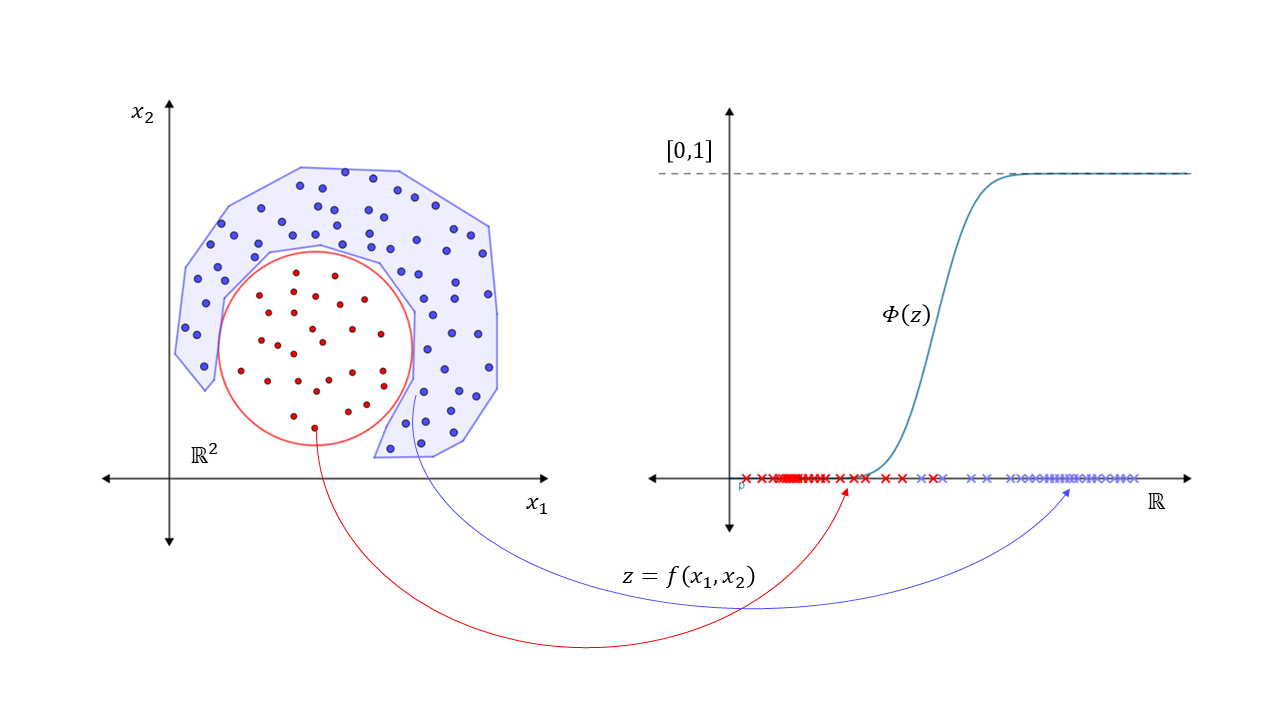
\includegraphics[width = 1\textwidth]{Diagrama_Separabilidad}
  \caption{Diagrama explicativo de un modelo de clasificación probit no lineal}
  \label{fig:DiagramaIntro}
\end{figure}

% De donde y cómo? se plantea la estructura del modelo el capítulo 2
Para llevar a cabo la construcción, se comienza con una extensa discusión teórica y matemática en el Capítulo \ref{cap:Modelo}. Dada su estructura, el modelo se puede estudiar de \textit{arriba hacia abajo}, es decir, de la parte más general a la parte más profunda. Por lo tanto, primero se estudian los Modelos Lineales Generalizados (GLM), específicamente los modelos probit asociados a la distribución normal. Los GLM dan el salto de una regresión donde la respuesta $y_i$ es real, a regresiones donde la respuesta puede ser discreta o restringida a cierto dominio \autocite{maccullagh1989generalized}. Los GLM, como su nombre lo indica, siguen siendo lineales en las covariables; sin embargo, se pueden flexibilizar usando las ideas de los Modelos Aditivos Generalizado (GAM) presentadas en \citet{hastie1986generalized}. En estos modelos, la flexibilización se lleva a cabo transformando a las covariables $\xsn_i$, previamente a la regresión, mediante la función $f$ usando métodos no paramétricos. Este trabajo, toma esas ideas y las combina con las de \citet{mallik1998automatic} en las que se modifica la transformación antes mencionada al darle una forma funcional concreta a $f$, correspondiente a una serie de polinomios por partes de continuidad y grado arbitrarios. La expansión resultante, tiene la peculiaridad que conectan muchas disciplinas y ramas de las matemáticas que han sido de mucha utilidad no sólo en el campo de la estadística. A lo largo del capítulo, se verá que con principios presentados, se abren las posibilidades en cuanto a modelos y datos sobre los que se pueden hacer regresiones. 

% Cómo se implement? Cap. 3
Desarrollado una vez el modelo, el Capítulo \ref{cap:BayesAlgoritmo} se concentra en su implementación. Para ello, se hace una breve introducción al paradigma bayesiano de la estadística, en particular al apredizaje bayesiano en un contexto de regresión lineal. Este paradigma, responde a que, usando las ideas de \citet{albert1993bayesian}, el algoritmo asociado al modelo recae en una técnica fundamental de la diciplina: el muestreador de Gibbs. Con esta poderosa herramienta, se presenta los detalles y lógica detrás de la implementación.
\begin{quote}
	\textit{[...], it is more common in machine learning to view the model as core, and how this is implemented
is secondary. From this perspective, understanding how to translate a mathematical model into a piece of
computer code is central.\footnote{\citet{barber2012bayesian}}}
\end{quote}
Asimismo, se explica a detalle el algoritmo, el cual se implementa en un paquete computacional para el lenguaje abierto de programación estadística\verb|R|.\footnote{El desarrollo y explicación del paquete de cómputo se detalla en el Apéndice \ref{ap:Paquete}, y corresponde a que, simplifica mucho el proceso de aprendizaje del modelo y fomenta su fácil uso y su validación por terceros. El paquete se puede descargar libremente de: \url{https://github.com/PaoloLuciano/bpwpm}}

% Cómo se probo? Cap. 4
Una vez que el modelo es funcional y fácil de implementar, en el Capítulo \ref{cap:EjYRes} se prueba y se valida contra una diversa serie de bases de datos. Primeramente, se hace una breve discusión sobre como evaluar la efectividad y precisión de un modelo como el presentado en este trabajo. Posteriormente, se corre el modelo contra cinco bases de datos simulados con dos covariables ($\xsn_i \in \mathbb{R}^2$). Estas pruebas preliminares, sirven para demostrar las capacidades predictivas del modelo y sobre todo, para hacer más concretas las matemáticas subyacentes y poder visualizar las diferentes fronteras flexibles obtenidas por el modelo. Asimismo, en este capítulo se discute la convergencia de las cadenas obtenidas del muestreador de Gibbs, uno de los puntos cruciales y delicados del modelo.\footnote{Como se verá en los capítulos subsecuentes, dada la expansión de $f$ en polinomios por partes, la \textit{identificabilidad} de los parámetros es uno de los puntos débiles del modelo.} Para cerrar el capítulo, se replica un escenario real de análisis y modelado, usando una base de datos médicos de cáncer de donde se obtienen excelentes resultados.

% Y luego? Conclusión Cap. 5
Finalmente, se cierra la discusión en el Capítulo \ref{cap:Conclusiones} donde se revisan consideraciones finales y limitantes del modelo, sin embargo, se abre una discusión a posibles extensiones para mejorarlo. Posteriormente, se da un rápido vistazo a modelos relativamente más modernos los cuales han sido capaces de proezas computacionales que se creían imposibles hace algunas décadas. No obstante, se verá que muchos de estos modelos más avanzados y usados hoy en día, son generalizaciones de modelos tradicionales. 
\end{document}